\chapter{Assurance Cases and Selected Evidence for AortaGeomRecon}

In this chapter, we discuss the scope of our work, which is building the evidence to support each claim of our AC  for \progname{}. The top level claims of the AC developed in previous work \cite{scs_ac} is correct and complete, thus we have a list of evidence that can support the arguments and the top level claims. Our work focus on providing the correct evidence for the assurance case, and the following material is presented: the Software Requirements Specification of \progname{}, the Design Document, the Module Guide, the Test Plan, the Algorithm Review,  the User Manual, the User Instruction Video, and a Warning  Message implemented  in \progname{}.

\section{Assurance Case Development}

Assurance Case is build with claims, subclaims, contexts and the evidence. The parts of  the AC  add up  to an argument for why the top level claim is true. By using Astah System Safety software to present the Goal Structuring Notation (GSN) arguments \cite{Astah_2023}\cite{kelly2004goal}, we want to show that our software delivers correct outputs when used for its intended use/purpose in its intended environment, and within its assumed operating assumptions. The Figure~\ref{fig_agr_ac_top} shows the top level of the assurance cases. With the goal of arguing that the software delivers correct outputs, we decompose the goal into 4 sub goals: GR, GI, GA and GBA, where GR stands for the goal of correct requirements of the software, GI stands for the goal of the implementation  matching the requirements, GBA is the goal of  that all  operational assumptions have been defined, and GA is the goal that all operational assumptions are met.

\begin{figure}[hp]
    \centering
    \fbox{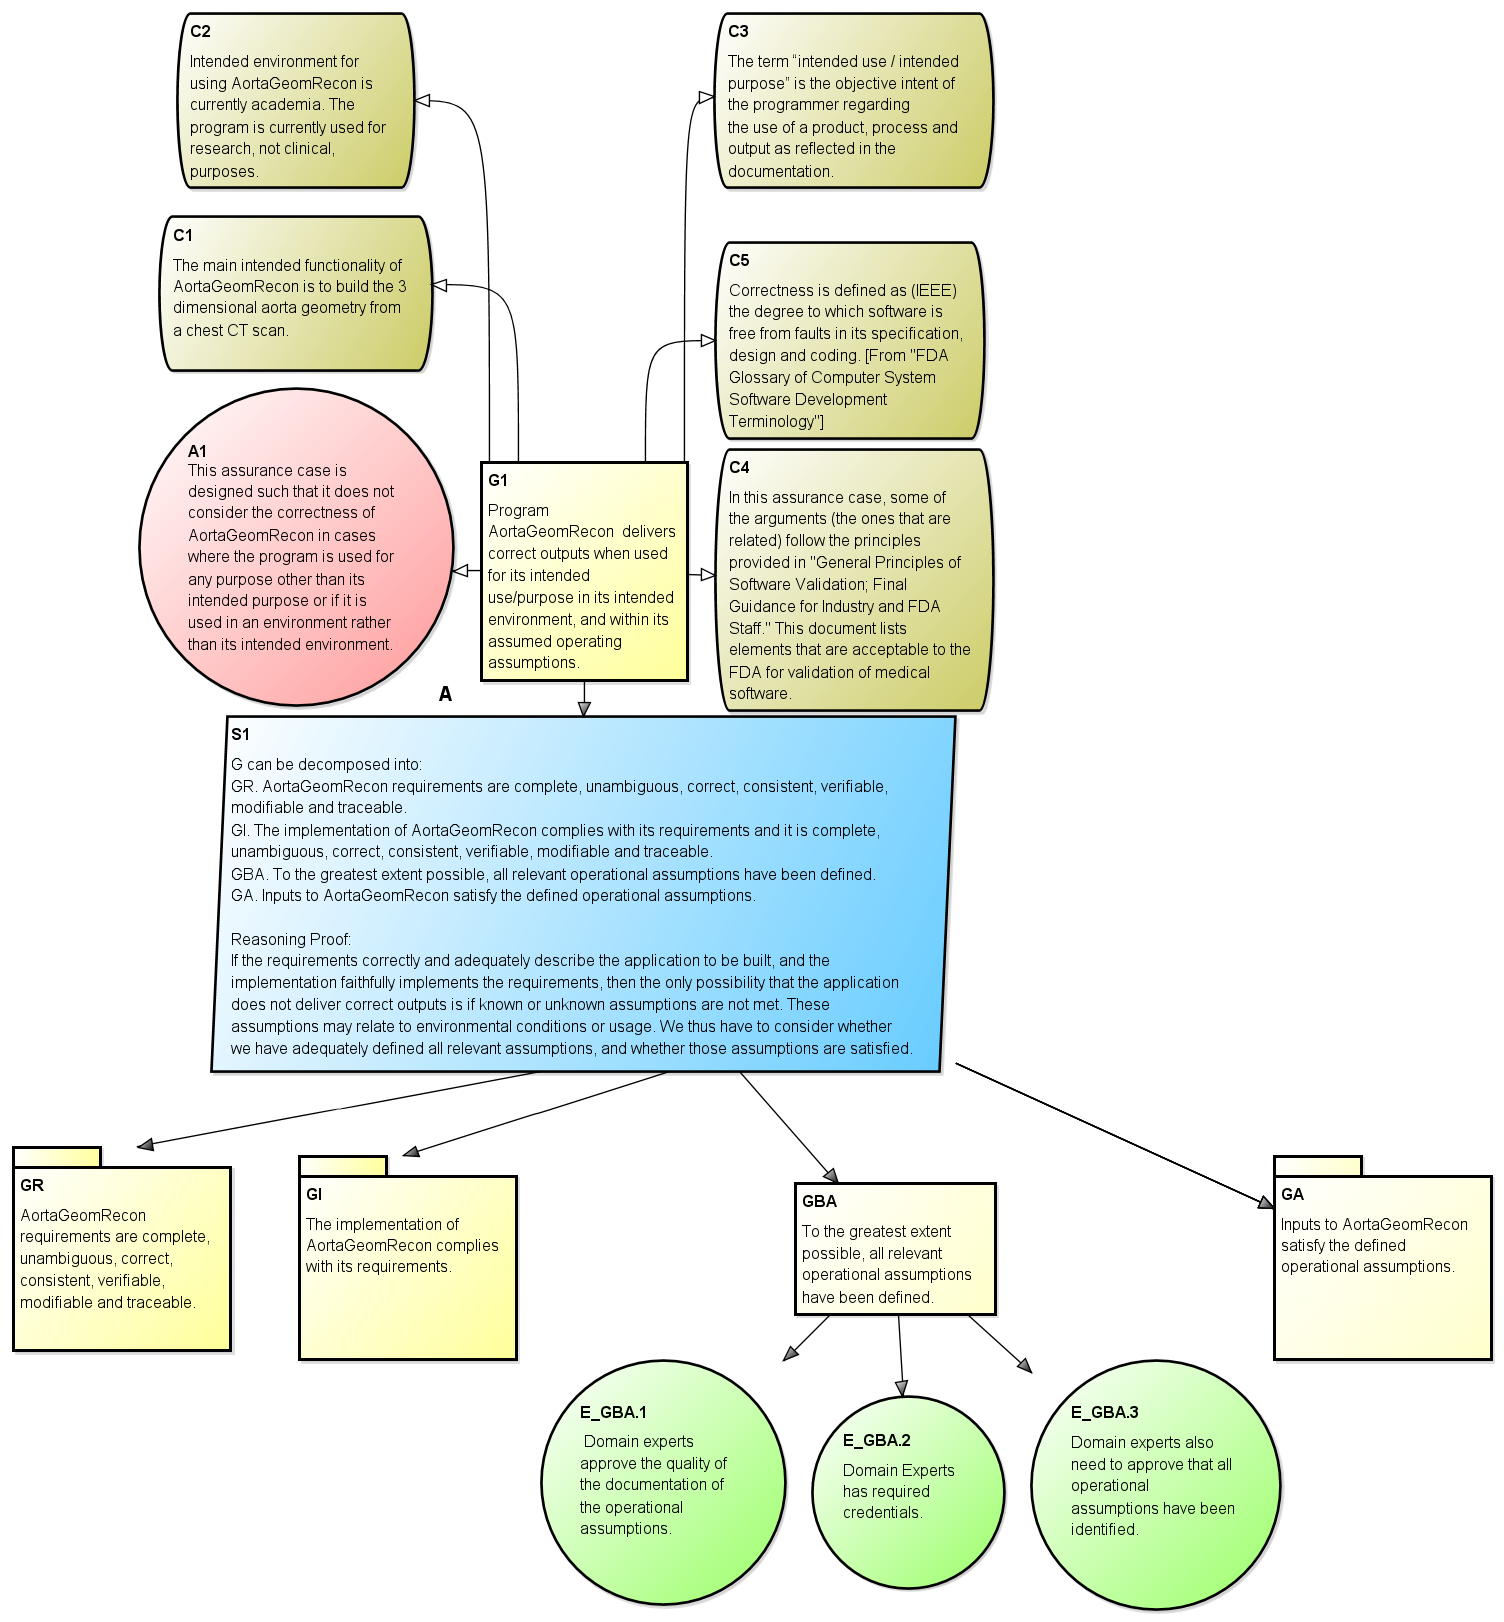
\includegraphics[width=0.99\textwidth]{figures/AC/Top_Level.png}}
    \caption[AortaGeomRecon Assurance Cases Top Level]{AortaGeomRecon Assurance Cases Top Level}
    \label{fig_agr_ac_top}
\end{figure}


\section{Assurance Case for Software Specification Requirements}

The first goal of getting a trusted software is having a complete, unambiguous, correct, consistent, verifiable, modifiable and traceable SRS that shows the complete breakdown of the requirements with mathematical notation, data models and instance models. The SRS is the foundation of the software development, and the design and the implementation will be based on the requirement document.

The Figure~\ref{fig_agr_ac_gr} demonstrates the claims on the goal of correct requirements of \progname{}. On the left branch, GR\_3C implies the goal of a complete, correct, and consistent documentation. Under this claim, the goal is separated based on each characteristic, and the corresponding evidence is presented as the leaf node. The S\_Correctness and S\_Completeness.4 node require a domain expert to review the quality of the document to ensure the documentation met the goal of the claims. The other characteristics of the documentation are supported with evidence as shown in the other branches in GR.

\begin{figure}[hp]
    \centering
    \fbox{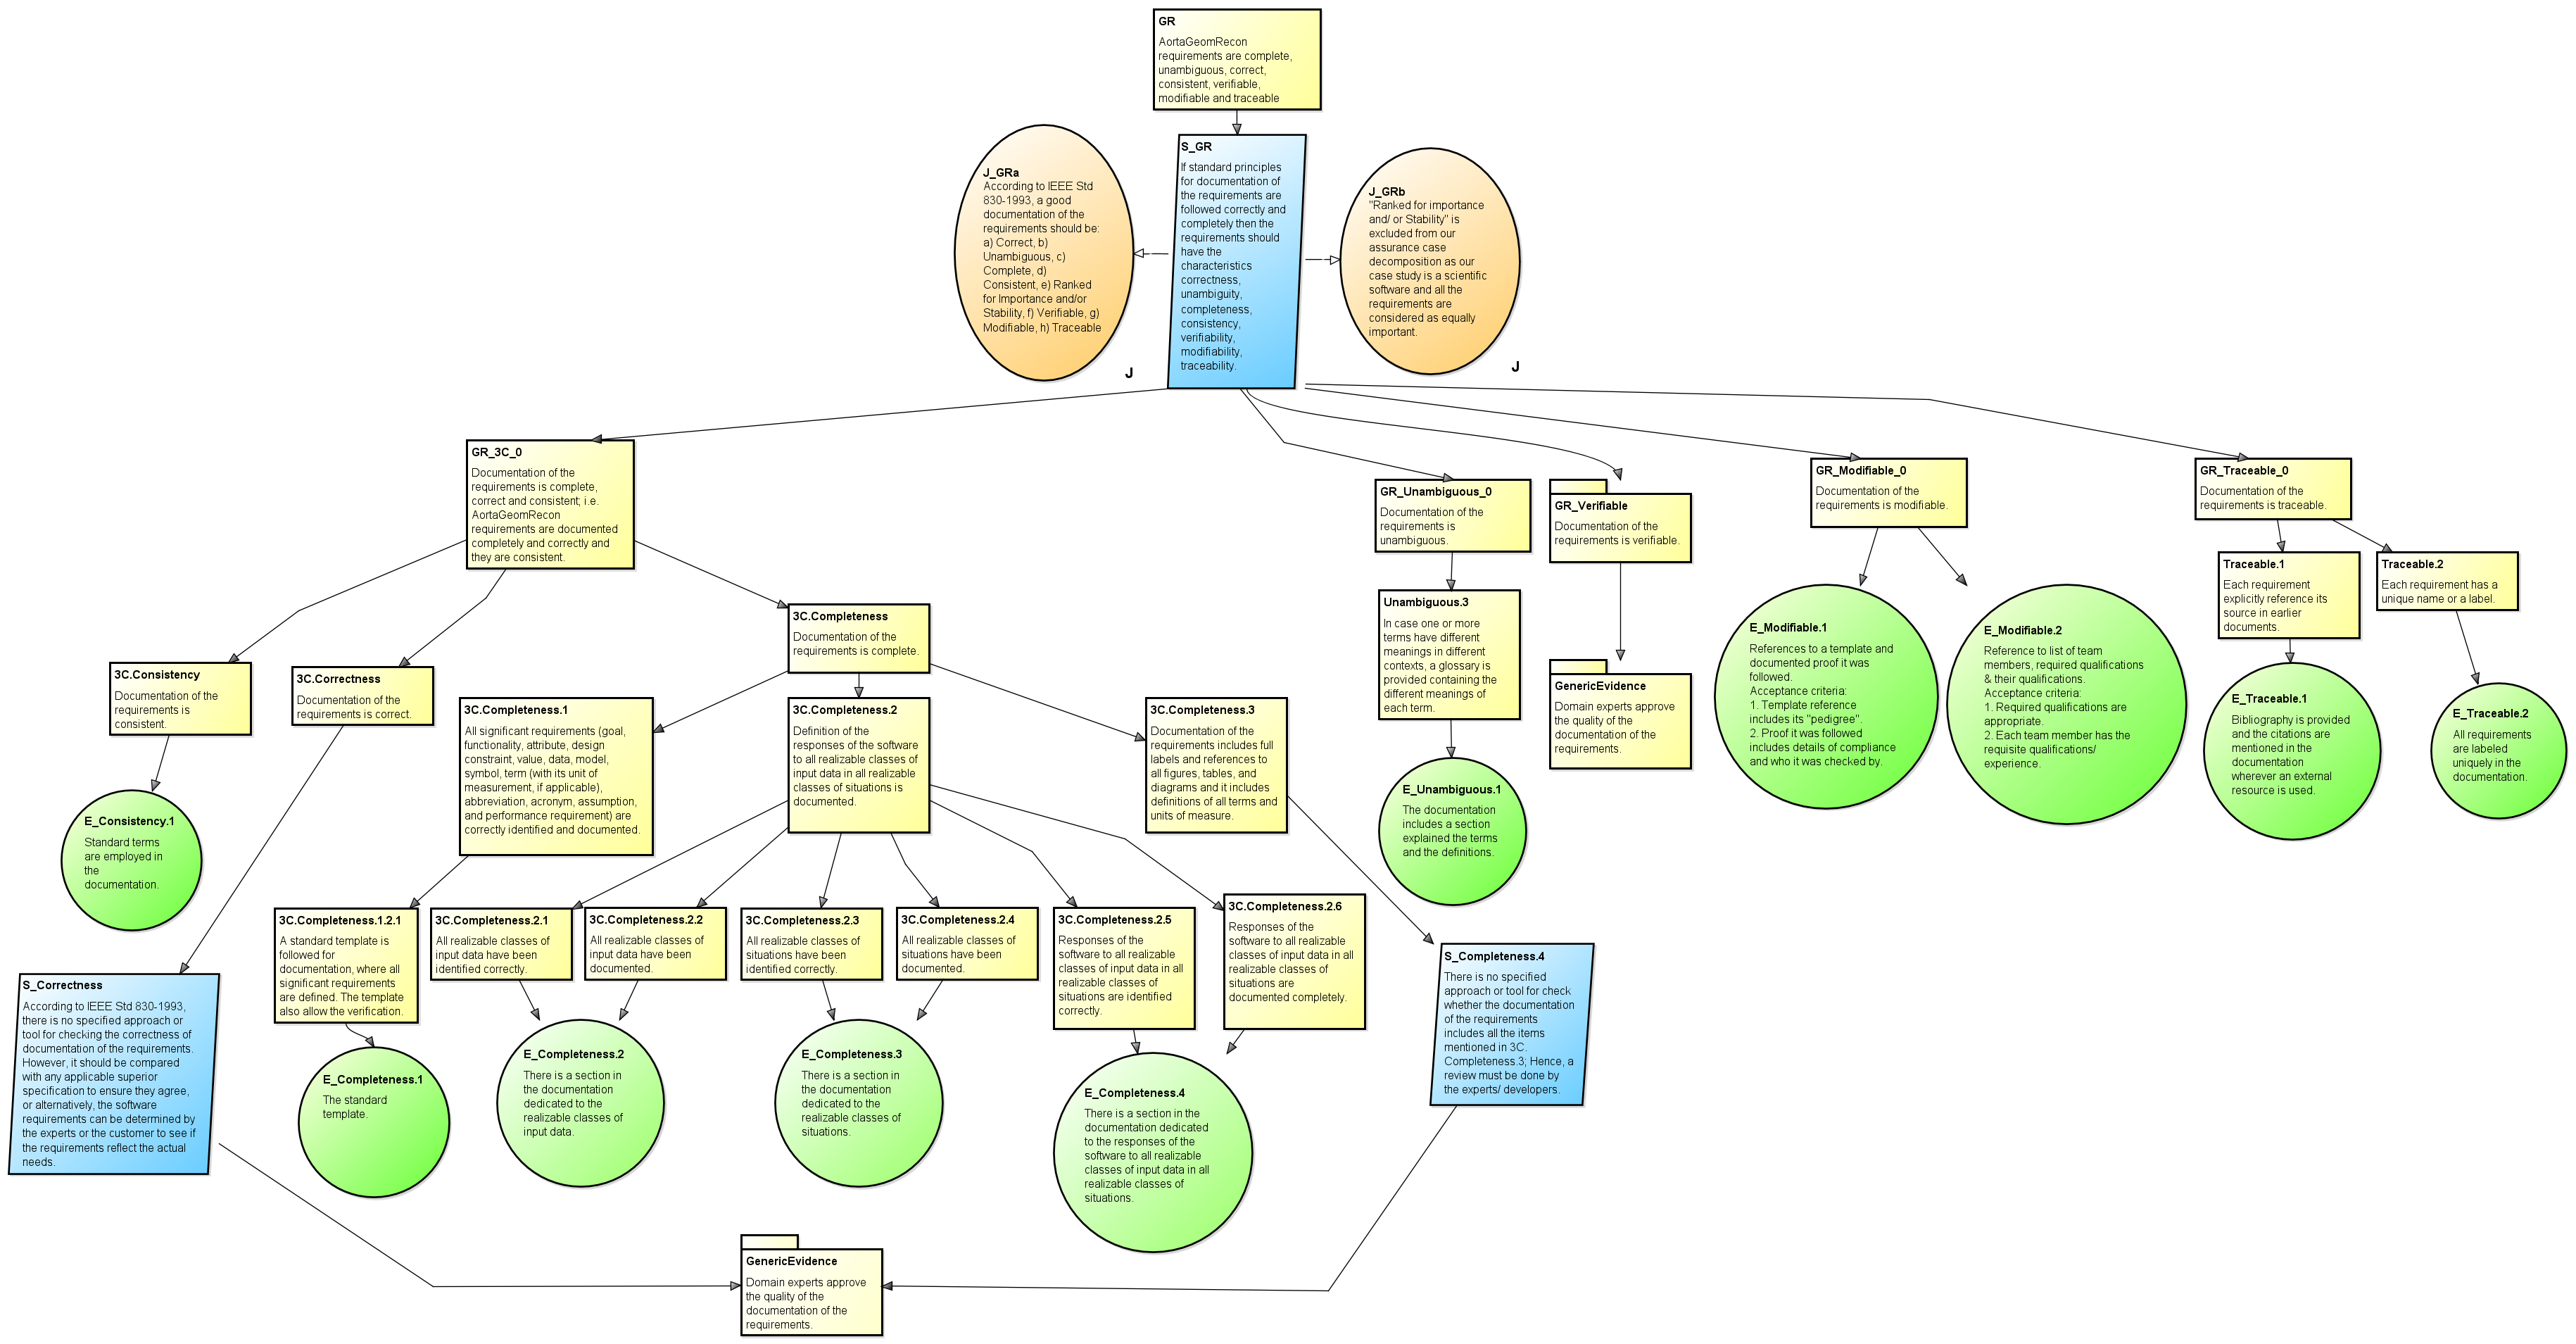
\includegraphics[width=1.3\linewidth, angle=90]{figures/AC/SRS/GSN_GR.png}}
    \caption[AortaGeomRecon Assurance Cases GR]{AortaGeomRecon Assurance Cases GR}
    \label{fig_agr_ac_gr}
\end{figure}

As explains in the assurance case GR, one of  most important statement of SRS having these characteristics is using a standard template. Using  a standard template means that all necessary requirements have been defined, and it allows a domain expert who has used this template to verify the quality of the document. We used a template tailored for research software \ref{Smith2006}, which is the standard template in the evidence E\_Completeness.1, and all other evidences where a template is included.

The chapters in the SRS and some of the most important sections in the chapter are explained below:
\begin{itemize}
\item Reference Material

In this section, a Table of Symbols and an Abbreviations and Acronyms table are used to explain every symbol and Abbreviations used in the SRS document. These tables ensure the consistency and the unambiguous characteristics of the document, as the evidences E\_Consistency.1 and E\_Unambiguous.1 shown in the Figure~\ref{fig_agr_ac_gr}. They are located at the very beginning of the document, so the reader will firstly look at these tables before reading the entire document. 

\item Introduction

In the introduction section, we introduced the problems and the scope of the document to the user by explaining the purpose of document, abstracting the scope of requirements and defining the characteristics of intended reader. This is provided for the reader to eliminates unambiguous in reading the document.

\item General System Description

The general system description includes a system context diagram which explains the relationship between the users, the inputs given by the user and the outputs of the AortaGeomRecon program. User responsibility and AortaGeomRecon responsibility are defined such that the reader knows what to do to successfully generate the desired result. 

\item Specific System Description

In this section, we are presenting more details about the problem and the specific system to solve the problem. The first subsection Problem Description discussed on the definition of Organ Segmentation, Coordinate Systems used in medical image problem, Physical System Description which is not available, and Goal Statements which is extract the three-dimensional segmentation of the aorta.

In the next subsection, Solution Characteristics Specification, we started with the assumptions to clearly define the scope of the requirement document, as shown in Figure~\ref{fig_agr_srs_a}. In the subsection Data Definitions, we defined Voxel, Image/Slice, and Volume with mathematical notation so that the developer can easily interpret. Next, in the subsection Instance Model, we showed the mathematical meaning of Region of Interest, and Segmentation, which are the two essential models that the developer must know in order to develop the solution.

\begin{figure}[H]
    \centering
    \fbox{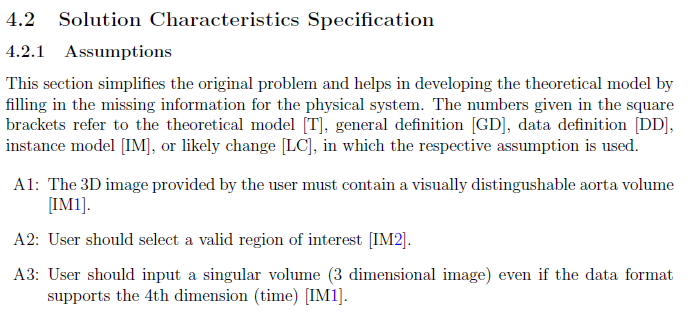
\includegraphics[width=\textwidth]{figures/AC/SRS/Assumptions.png}}
    \caption[AortaGeomRecon SRS Assumptions]{AortaGeomRecon SRS Assumptions}
    \label{fig_agr_srs_a}
\end{figure}


\item Requirements

With all the information in the document, we can now present the Functional Requirements and the Non-Functional Requirements for the program AortaGeomRecon. The Functional Requirements are defined by using the terms we presented in Data Definitions, Instance Model, and based on the other Functional Requirements, as shown in Figure~\ref{fig_agr_fr}. The Non-Functional Requirements usually have a measurement such as execution time, the effort of manual works, etc.

\begin{figure}[H]
    \centering
    \fbox{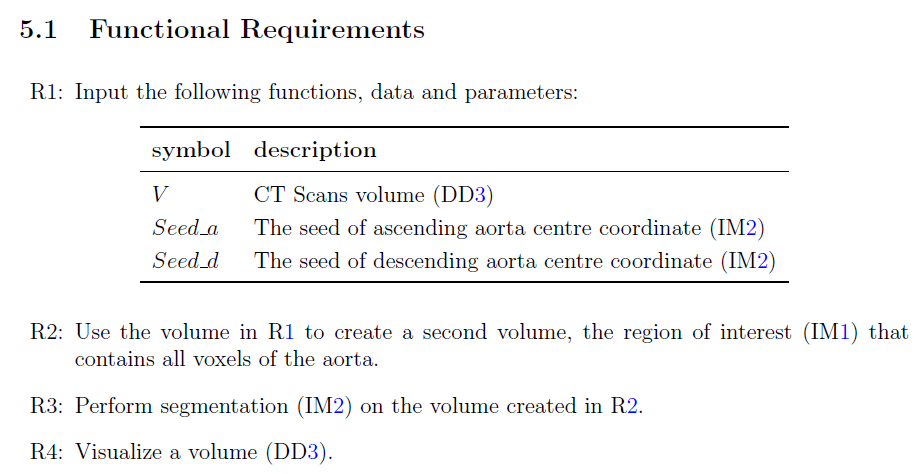
\includegraphics[width=0.75\textwidth]{figures/AC/SRS/Functional_Requirements.png}}
    \caption[AortaGeomRecon Functional Requirements]{AortaGeomRecon Functional Requirements}
    \label{fig_agr_fr}
\end{figure}

\begin{figure}[H]
    \centering
    \fbox{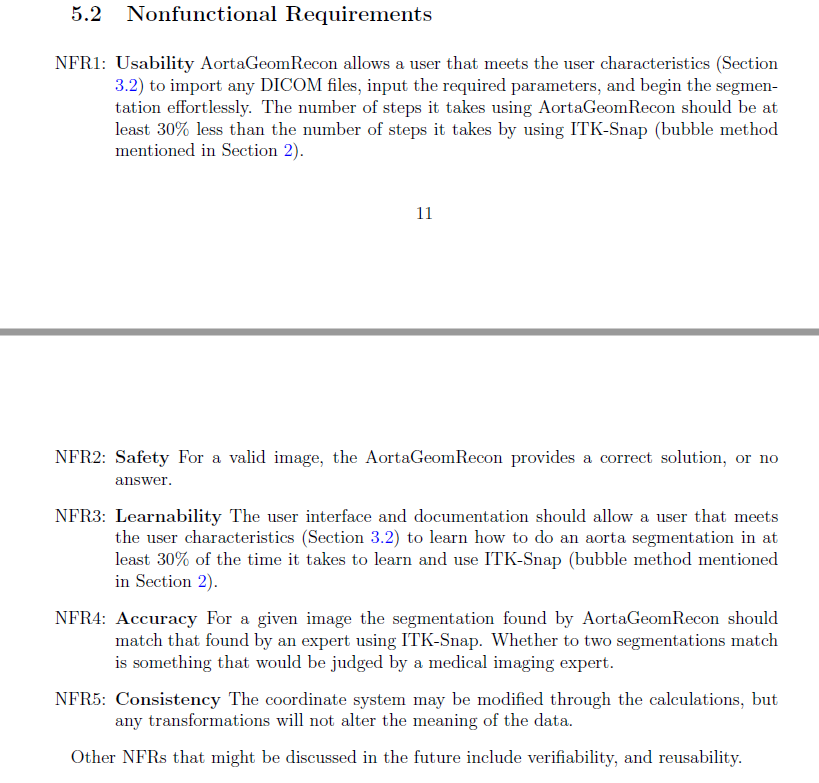
\includegraphics[width=0.75\textwidth]{figures/AC/SRS/NonFunctional_Requirements.png}}
    \caption[AortaGeomRecon Non- Functional Requirements]{AortaGeomRecon Non- Functional Requirements}
    \label{fig_agr_nfr}
\end{figure}

\item Likely Changes and Unlikely Changes

This section discussed the likely changes that the developer might expect a change in the future works, and the unlikely changes that is most certainly not going to change for a justified reason. The only likely change discussed in the AortaGeomRecon's SRS is regarding the segmentation method. For different segmentation method, the inputs varies, since the segmentation method is a likely change, the inputs variables are also likely changes. The only unlikely change is the method of retrieve a region of interest. Most methods take a starting point and sizes in different dimensions to get the region of interest.

\item Traceability Matrix and Graphs

The traceability matrices are to provide easy references on what has to be additionally modified if a certain component is changed. Below shows the traceability matrices of different sections:
\begin{figure}[H]
    \centering
    \fbox{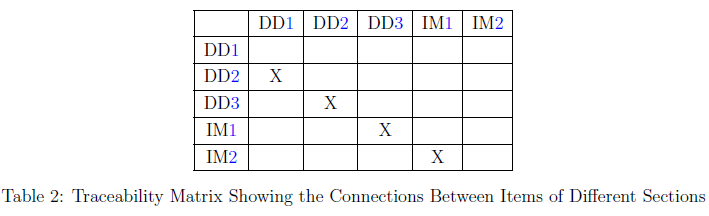
\includegraphics[width=\textwidth]{figures/AC/SRS/tm_dd_im.png}}
    \caption[AortaGeomRecon Traceability Matrix between Data Definitions and Instance Model]{AortaGeomRecon Traceability Matrix between Data Definitions and Instance Model}
    \label{fig_agr_tm_dd_im}
\end{figure}

\begin{figure}[H]
    \centering
    \fbox{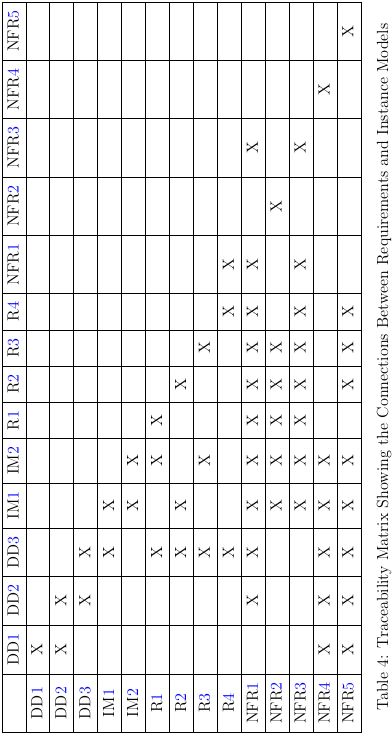
\includegraphics[width=\textwidth]{figures/AC/SRS/tm_im_r.png}}
    \caption[AortaGeomRecon Traceability Matrix Between Requirements and Other sections]{AortaGeomRecon Traceability Matrix Between Requirements and Other sections}
    \label{fig_agr_tm_im_r}
\end{figure}

\begin{figure}[H]
    \centering
    \fbox{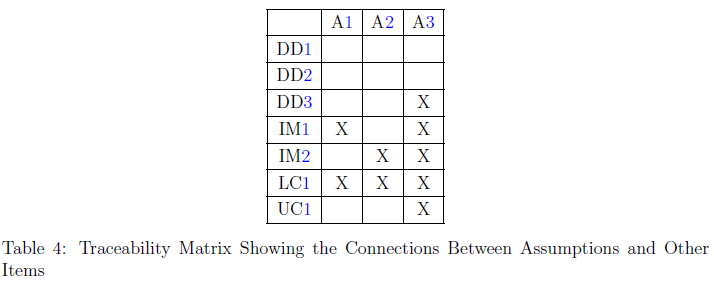
\includegraphics[width=\textwidth]{figures/AC/SRS/tm_a.png}}
    \caption[AortaGeomRecon Traceability Matrix Between Assumptions and Other sections]{AortaGeomRecon Traceability Matrix Between Assumptions and Other sections}
    \label{fig_agr_tm_a}
\end{figure}


\end{itemize}

\section{Assurance Case for Implementation}
The goal of implementation asked the developer to fully comply the design and the implementation with the Software Requirements Specification document. Since we have showed with Assurance Case that our SRS is complete, consistent, and unambiguous, the design and the implementation that fully complying with requirements is correct.

\begin{figure}[H]
    \centering
    \fbox{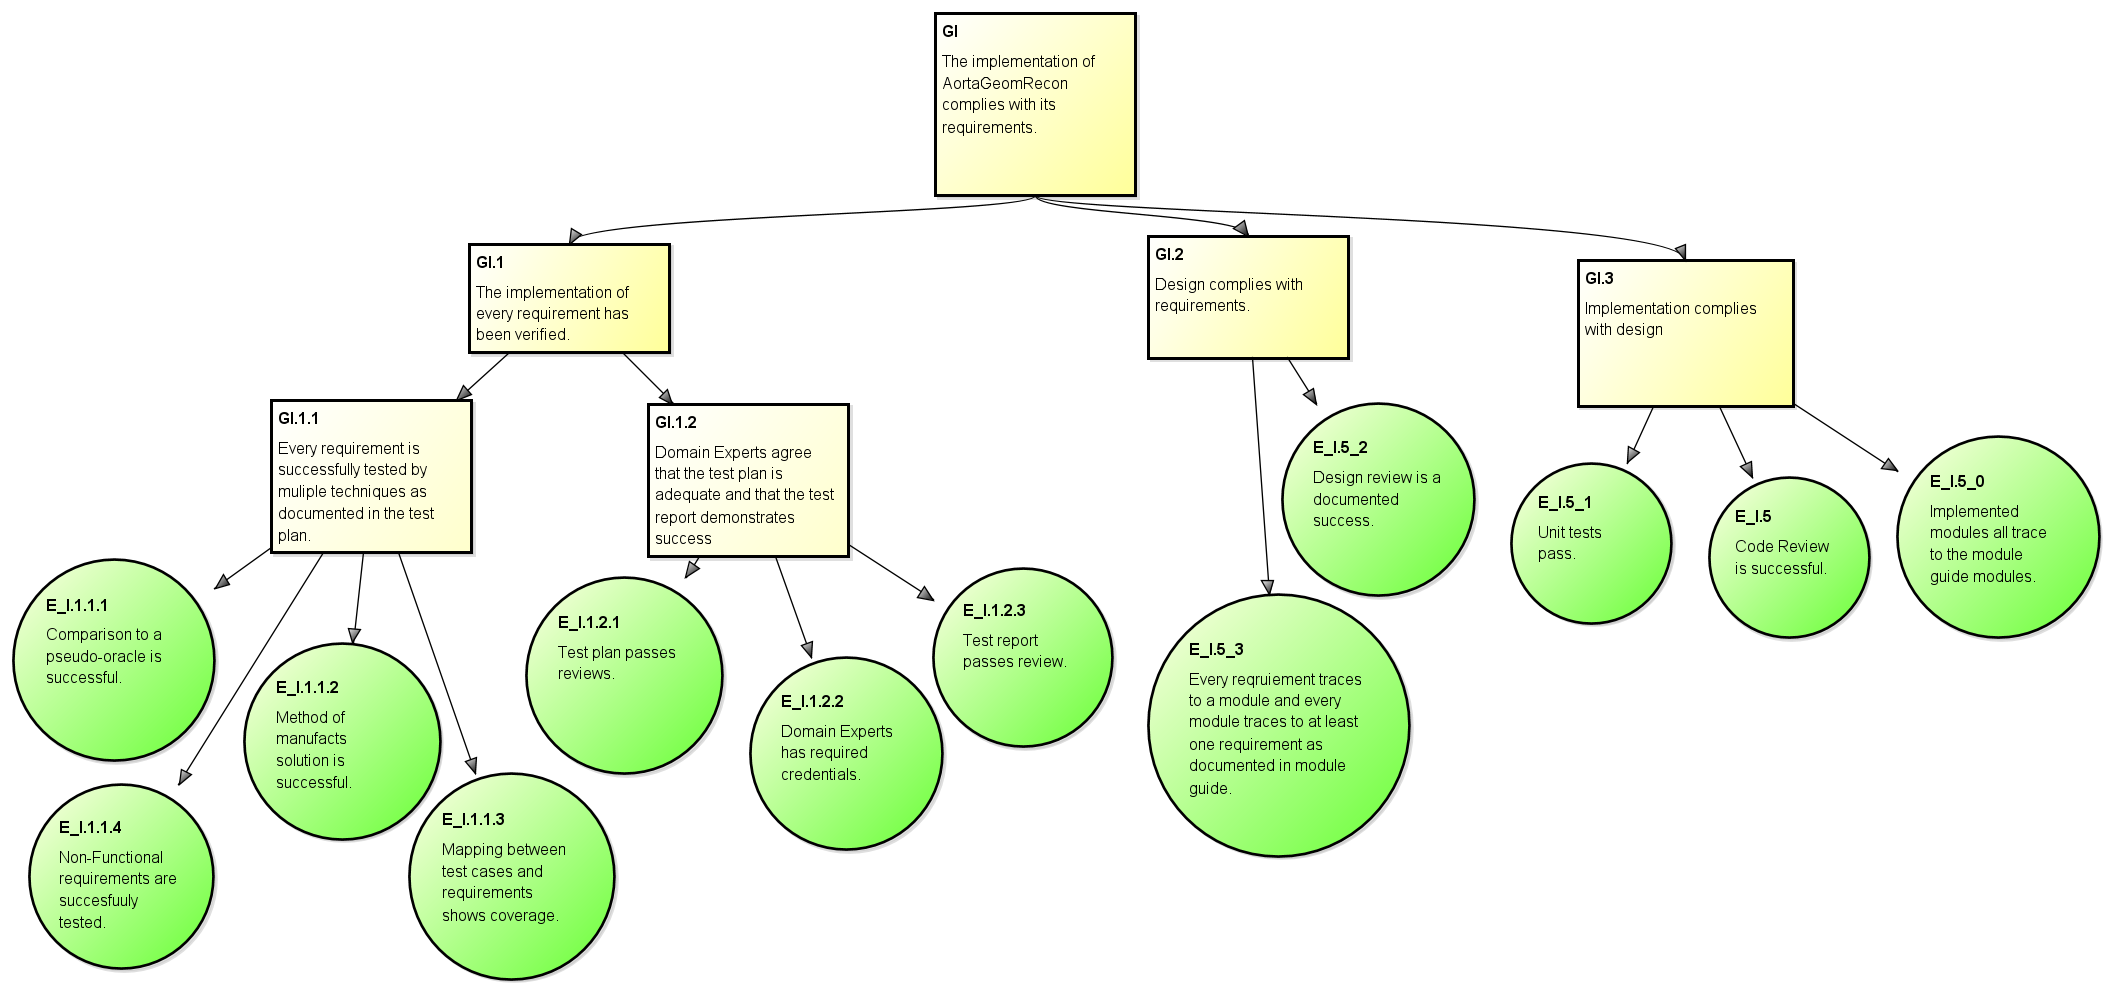
\includegraphics[width=\textwidth]{figures/AC/GI/GSN_GI.png}}
    \caption[AortaGeomRecon Assurance Cases For Implementation]{AortaGeomRecon Assurance Cases For Implementation}
    \label{fig_agr_ac_gi}
\end{figure}

\subsection{Design Document}
The purpose of the Design Document \cite{DD} is to explain in details how the algorithm works, and why it worked. Similar to what section \ref{algo} wrote, the design document explains in plan text the workflow of the algorithm. The design document is a piece of evidences that demonstrate unambiguity characteristic.

\subsubsection{Sphinx - Python Documentation Generator}
To implement this Design Document, I used Sphinx, a Python Documentation Generator that can build module's documentation with the comments in the source code. Moreover, using reStructuredText to write the Algorithm Overview, we can build HTML binary which can be published on a web server. Another important section in Design Document is the Glossary. It has rich vocabulary explanation, images, and links to the outside source to let the reader understands as much as possible.

\begin{figure}[H]
    \centering
    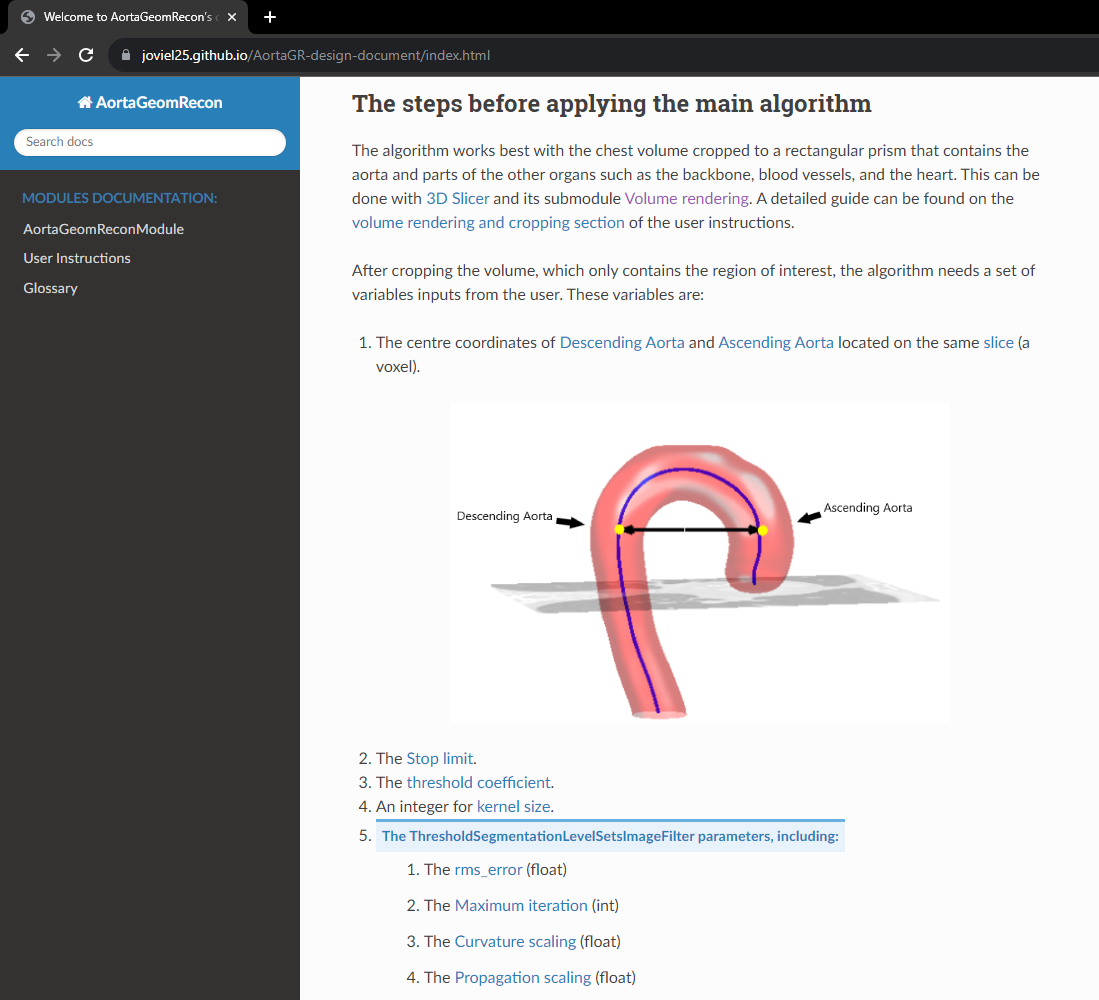
\includegraphics[width=0.9\textwidth]{figures/AC/DD/Main_page.png}
    \caption[AortaGeomRecon Design Document Website]{AortaGeomRecon Design Document Website}
    \label{fig_agr_dd}
\end{figure}

\begin{figure}[H]
    \centering
    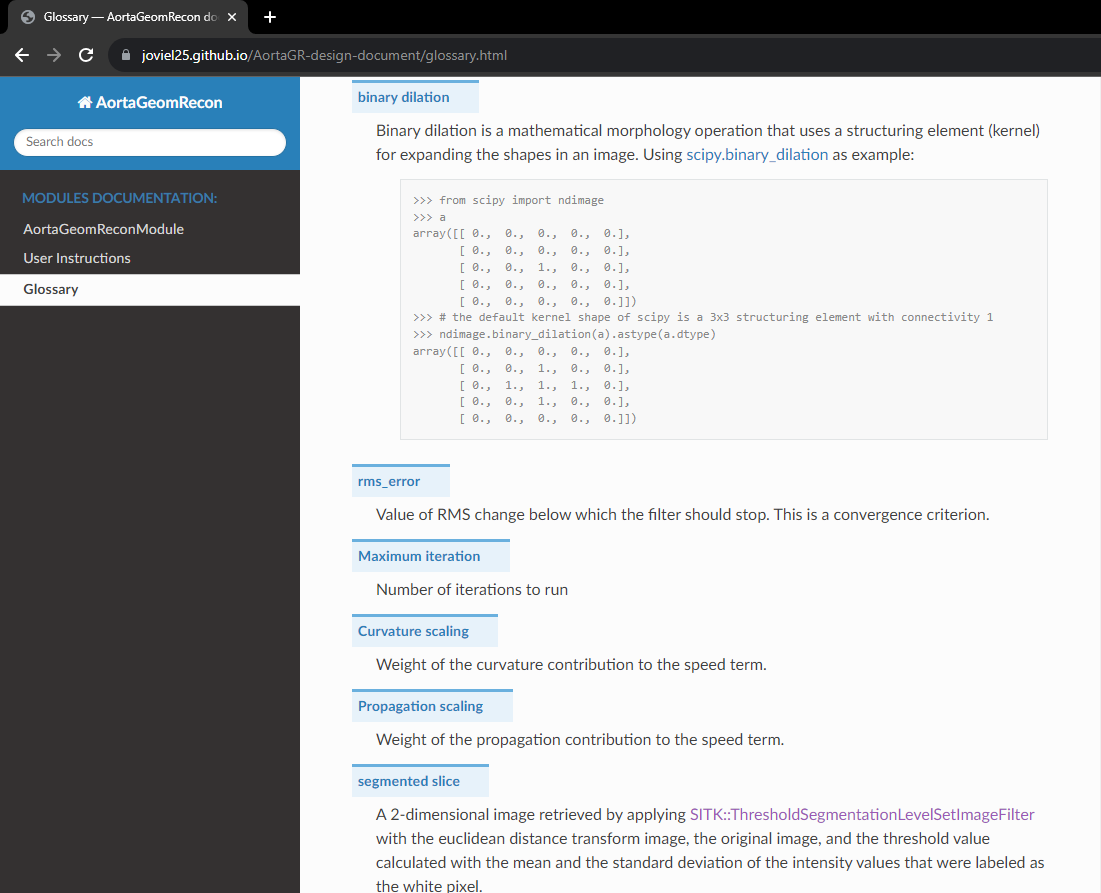
\includegraphics[width=\textwidth]{figures/AC/DD/Glossary.png}
    \caption[AortaGeomRecon Design Document Glossary]{AortaGeomRecon Design Document Glossary}
    \label{fig_agr_dd_glossary}
\end{figure}

\subsection{Module Guide}

Another important documentation to show that the design is complete, correct, and consistent design is Module Guide. In the design of the software, we first list the anticipated changes such that we are expecting a change to this piece of requirement of information, we will keep it a single module so when the changes did happen, we only need to concern about the module and its dependency modules. The anticipated changes are listed in the Figure~\ref{fig_agr_ac} below.

\begin{figure}[H]
    \centering
    \fbox{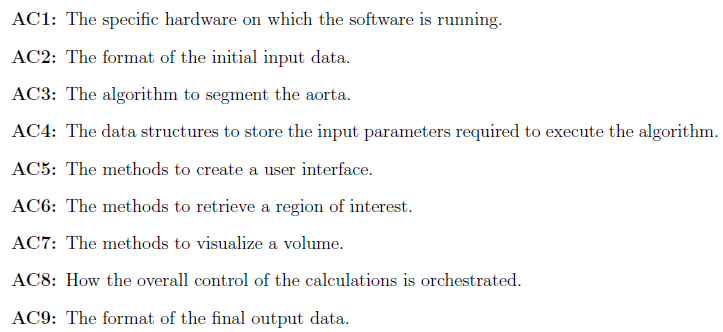
\includegraphics[width=\textwidth]{figures/AC/MG/Anticipated_Changes.png}}
    \caption[AortaGeomRecon Anticipated Changes]{AortaGeomRecon Anticipated Changes}
    \label{fig_agr_ac}
\end{figure}

Modules are decomposed according to the principle of “information hiding” proposed by Parnas et al. (1984). The Secrets' field in a module decomposition is a brief statement of the design decision hidden by the module. The Services' field specifies what the module will do without documenting how to do it. For each module, a suggestion for the implementing software is given under the Implemented By title. If the entry is OS, this means that the module is provided by the operating system or by standard programming language libraries. AortaGeomRecon means the module will be implemented by the AortaGeomRecon software.

\begin{figure}[H]
    \centering
    \fbox{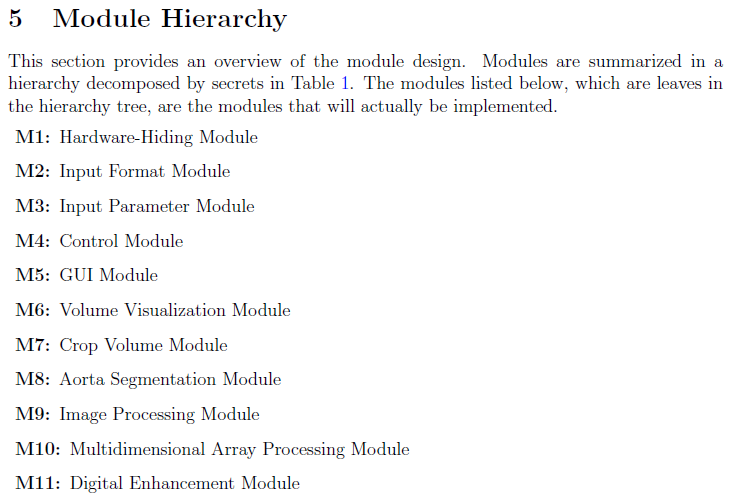
\includegraphics[width=\textwidth]{figures/AC/MG/Modules.png}}
    \caption[AortaGeomRecon Modules]{AortaGeomRecon Modules}
    \label{fig_agr_modules}
\end{figure}

\begin{figure}[H]
    \centering
    \fbox{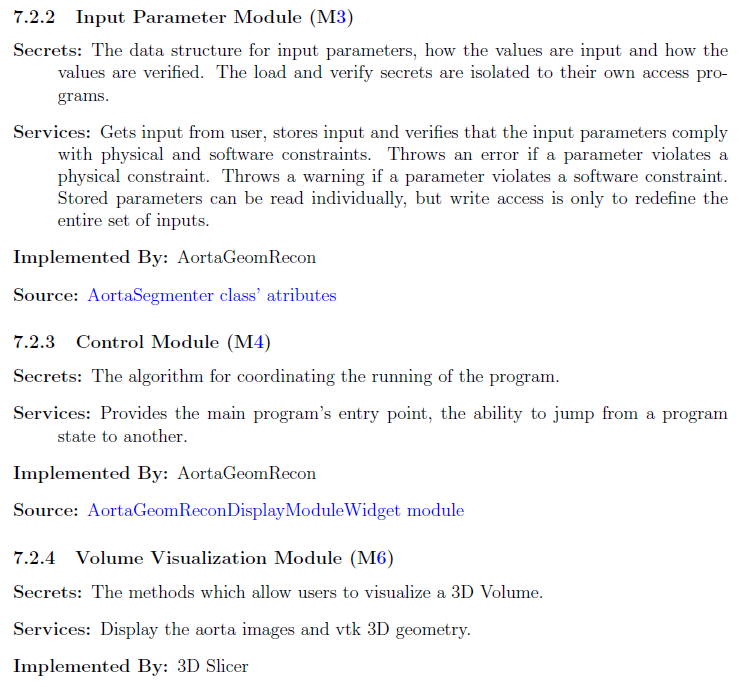
\includegraphics[width=\textwidth]{figures/AC/MG/Modules_Decomposition.png}}
    \caption[AortaGeomRecon Module Decomposition Example]{AortaGeomRecon Module Decomposition Example}
    \label{fig_agr_md}
\end{figure}

Now that we have listed the anticipated changes and the modules, we are using traceability matrices to show the relationships between the modules and the anticipated changes, and the modules between the requirements. This indicates that the design is fully complying with the requirements, as we stated in GI.2 in the Figure~\ref{fig_agr_ac_gi}.

\begin{figure}[H]
    \centering
    \fbox{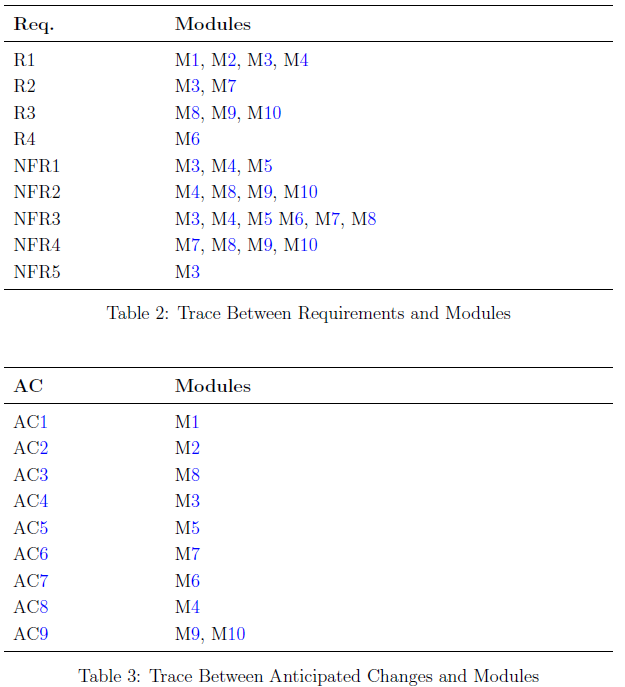
\includegraphics[width=\textwidth]{figures/AC/MG/TM.png}}
    \caption[AortaGeomRecon Modules Traceability Matrices]{AortaGeomRecon Modules Traceability Matrices}
    \label{fig_agr_mtm}
\end{figure}

On top of relating the modules to the requirements, we are relating the actual source code to the modules, which is a strong evidence of our implementation has fully complying with the requirements. Since our requirements has proven to be correct, complete, and consistent, the implementation must also be trustworthy.

\begin{figure}[H]
    \centering
    \fbox{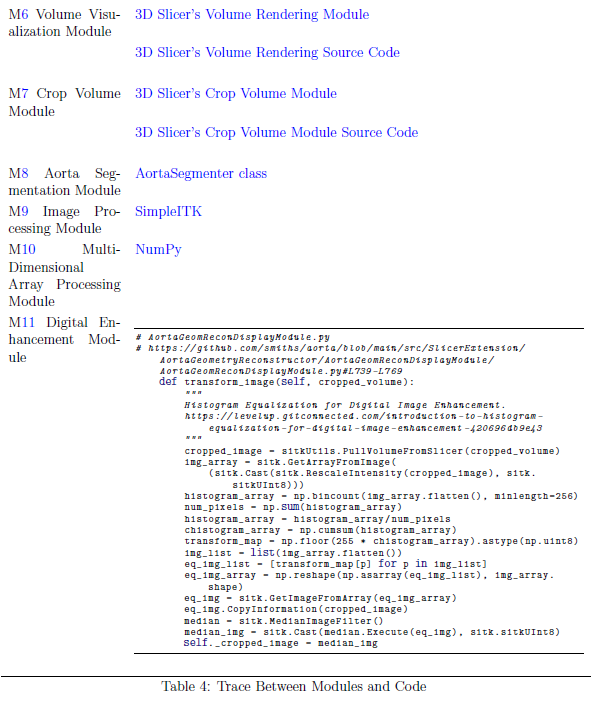
\includegraphics[width=0.9\textwidth]{figures/AC/MG/TM_modules_code.png}}
    \caption[AortaGeomRecon Part Of The Traceability Matrix On Modules And Code]{AortaGeomRecon Part Of The Traceability Matrix On Modules And Code}
    \label{fig_agr_mtm_modules_code}
\end{figure}

\subsection{Test Plan}

GI.1.2 claim states that a test plan must be adequate and test report demonstrates success. Unlike the other algorithm that can easily be tested with a ground truth test case, our ground truth case is build by using another more accurate method such as ITK-Snap's bubble method, then manually erase the unwanted pixels.

\subsubsection{Build "Ground Truth" data}
Instead of using ITK-Snap's bubble method, we build ground truth test case with our existing algorithm and updated algorithm. If there exists a difference between two results, our domain experts can make a visual comparison of both test cases to see which algorithm to use for the future.

\subsubsection{GitHub Actions workflows}
This leads to our Continuous Integration infrastructure, implemented with GitHub Actions workflow. A workflow is a configurable and automated process that will run one or more jobs on the desired system. GitHub Actions workflow used a YAML file to define the events and the commands to be executed on the temporary system, which has the build of the repository. \cite{GitHubActions}

We have set up two automated process which happens on each "push" event and "pull" event. A "push" event implies that something is changed in one or multiple commits, therefore there is a need to verify whether the commits have bugs that need extra fixes. A "pull" event happens when a feature branch is going to merge with the main branch. Since our main branch is protected, any update to the main branch must be merged by using a pull-request. Before a pull-request can be approved, the continuous integration tests are examined and until there are no errors, a pull-request cannot be merged with the main branch. 

The first automated process is a linter. A linter is a tool for static code analysis to flag programming errors, bugs, stylistic errors and suspicious constructs. We used Python Flake8 as our linter to find bugs and errors, and ensures that program's readability by striking the source code with Google's published  Python Style Guide. \cite{Linter}

The second automated process is our continuous integration tests. By setting up Git Large File System (LFS) and upload to pre-build ground truth test data in the repository, we can now pass the cropped volume as the inputs' data, the same Aorta seeds and the hyperparameters that we have used to generate the ground truth test data to the algorithm and verify the results. To compare the volumes, we used Dice similarity coefficient.

\subsection{Algorithm Review}

The algorithm review was an idea started with Code Walkthrough. A code walkthrough is one of the methods that can increase the participants' confidence, or finding program's bugs or error. For an Algorithm Review, we have not discussed what the program should do; we are presenting the algorithm to the domain expert and asking them if the design and implementation fulfill the implementation objectives.

\subsubsection{Tool used in Algorithm Review}

Spyder is a free and open source scientific environment written in Python, for Python, and designed by and for scientists, engineers and data analysts. The Variable Explorer allows the user to interactively browse the variables and the objects in debugging mode \cite{Spyder}
.
\begin{figure}[H]
    \centering
    \fbox{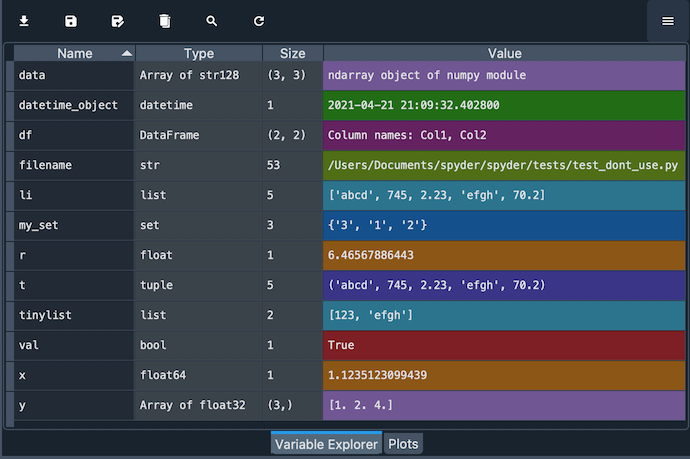
\includegraphics[width=0.8\textwidth]{figures/AC/AR/variable-explorer-standard.png}}
    \caption[Spyder Variable Explorer]{Spyder Variable Explorer \cite{raybaut2009spyder}}
    \label{fig_spyder_ve}
\end{figure}

This feature allows us to execute the program step by step, and see what happens to the variable (segmentation result) when executing the segmentation algorithm. 


\subsubsection{Algorithm Review with Kailin Chu}
The first algorithm review was done with Kailin Chu, who is a biomedical engineering student and started working the semi-automacial aorta segmentation algorithm as a summer researcher. Along with Smith Spencer, we were aiming to increase our confidence in this code walkthrough. This code walkthrough did not increase our confidence in the software, because the code was developed by Kailin from two years ago, so some details and design decisions are missing, and some variables were decided by trial and error. Despite that the code walkthrough has turned into an algorithm review, and it did not achieve what we wanted in the first place, this meeting was still very helpful. Knowing that the algorithm was partially based on trial and error, I was able to improve the algorithm and reaching a better result in a more efficient way.

\subsubsection{Algorithm Review with Dr. Dean Inglis}

The second algorithm review was conducted with Dr. Dean Inglis, an experienced professor, Medical Image Analyst, and Software Developer. We presented our segmentation algorithm to him and requested validation of our approach or suggestions for a potentially superior algorithm. Dr. Dean Inglis provided his insights on the algorithm, which we meticulously recorded on the GitHub issue tracker. These insights will guide the developer responsible for enhancing the program. This meeting significantly reinforced our confidence in both the software and our endeavors, whether the idea of developing an extension module for 3D Slicer or the algorithm itself.

\section{Assurance Case for Operational Assumptions}

\begin{figure}[H]
    \centering
    \fbox{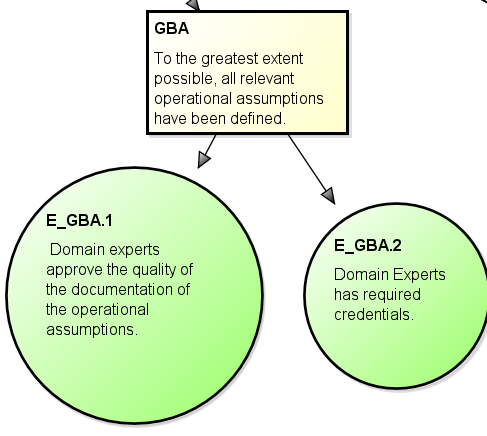
\includegraphics[width=0.3\textwidth]{figures/AC/GBA/GBA.png}}
    \caption[AortaGeomRecon Assurance Case Operational Assumptions]{AortaGeomRecon Assurance Case Operational Assumptions}
    \label{fig_agr_ac_gba}
\end{figure}

The evidence for the statement "To the greatest extent possible, all relevant operational assumptions have been defined" is quite simple as only Domain experts/customers approve the quality of the documentation. However, finalizing this evidence takes many efforts from the beginning of the project to the end of the project, because we want to continuously improve the quality of the content matching the most recent updates of the software.

\subsection{User Manual}
A user manual serves the purpose of documenting the all operational assumptions. When the user getting unexpected results by using this software, they can always refer to the user manual to see what pieces are different. Our user manual is initially located in GitHub repo's README, which is only available to the developers invited as the contributors. The content includes the installation of the software, importing the extension modules, import inputs data, and perform segmentation. The user manual is also available publicly on the design document website, assuming that the users might not be the repository contributors.

\begin{figure}[H]
    \centering
    \fbox{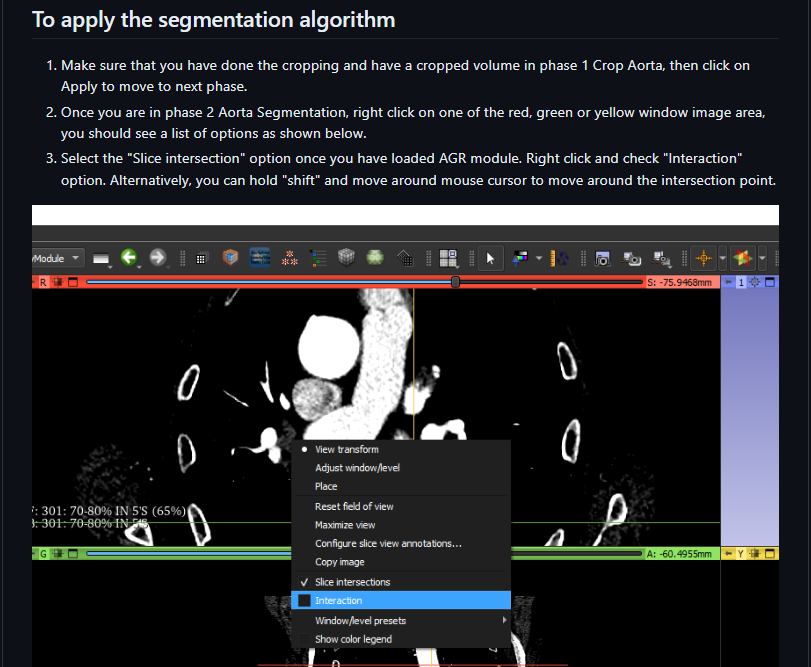
\includegraphics[width=0.9\textwidth]{figures/AC/GBA/User_manual.png}}
    \caption[AortaGeomRecon User Manual On GitHub README]{AortaGeomRecon User Manual On GitHub README}
    \label{fig_agr_git_um}
\end{figure}


\subsection{User Instruction Video}
Videos are an effective way to engage your audience and deliver information in a way that's easy to follow along and understand. A better instructional content is a YouTube Video where I make step-by-step instruction with voice over to instruct user. The video is not listed publicly on YouTube, but the users who have access to the GitHub repository or Design Document website can access this video by the URL link.

\begin{figure}[H]
    \centering
    \fbox{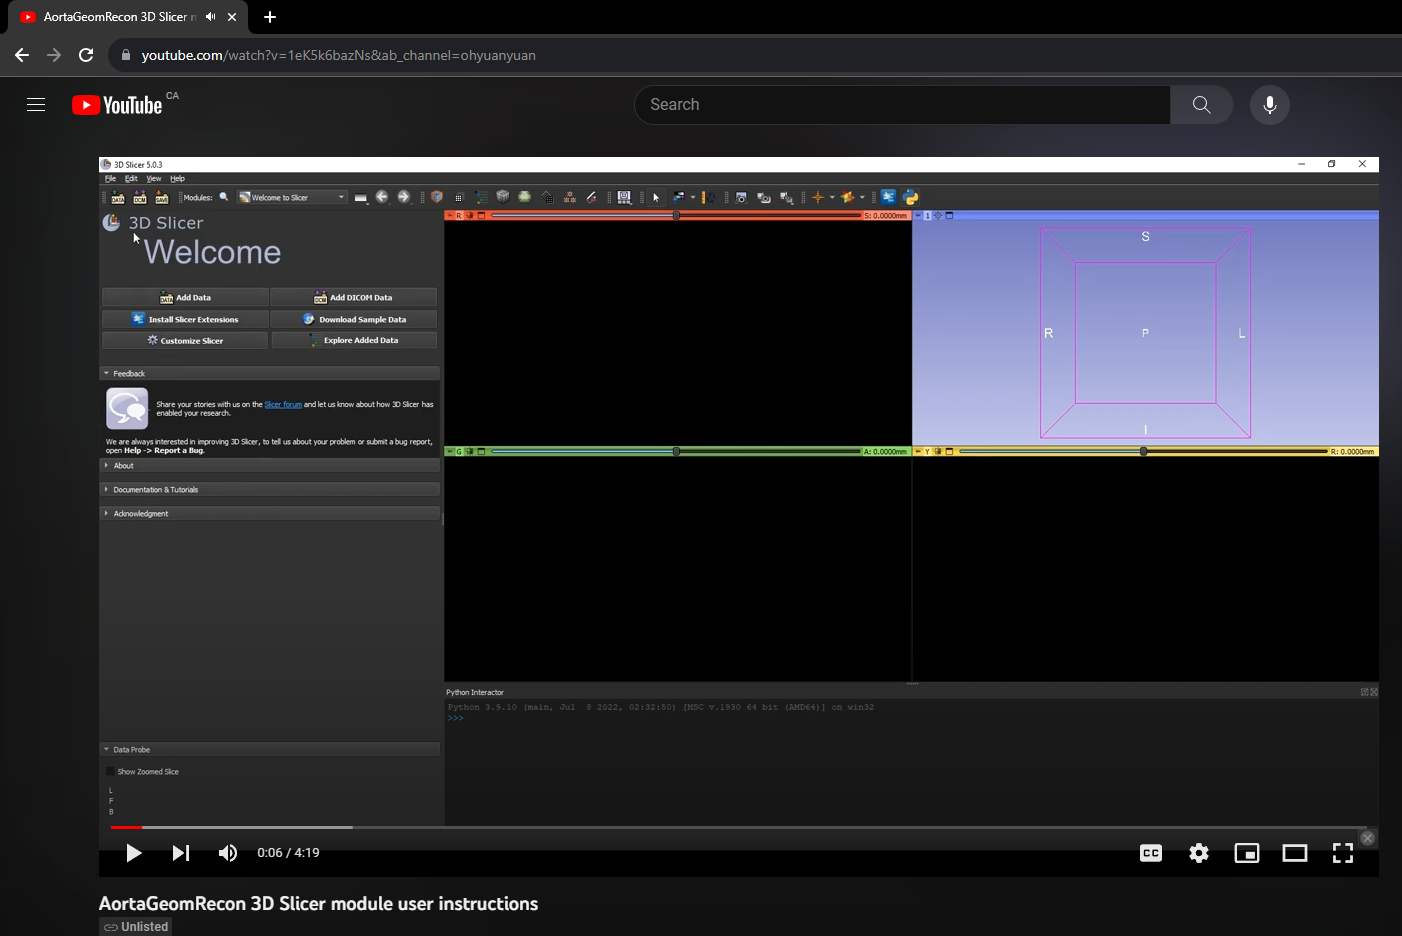
\includegraphics[width=0.8\textwidth]{figures/AC/GBA/User_instructions_video.png}}
    \caption[AortaGeomRecon User Instructions on YouTube]{AortaGeomRecon User Instructions on YouTube}
    \label{fig_video}
\end{figure}


\section{Assurance Case for Inputs Assumptions}

\begin{figure}[H]
    \centering
    \fbox{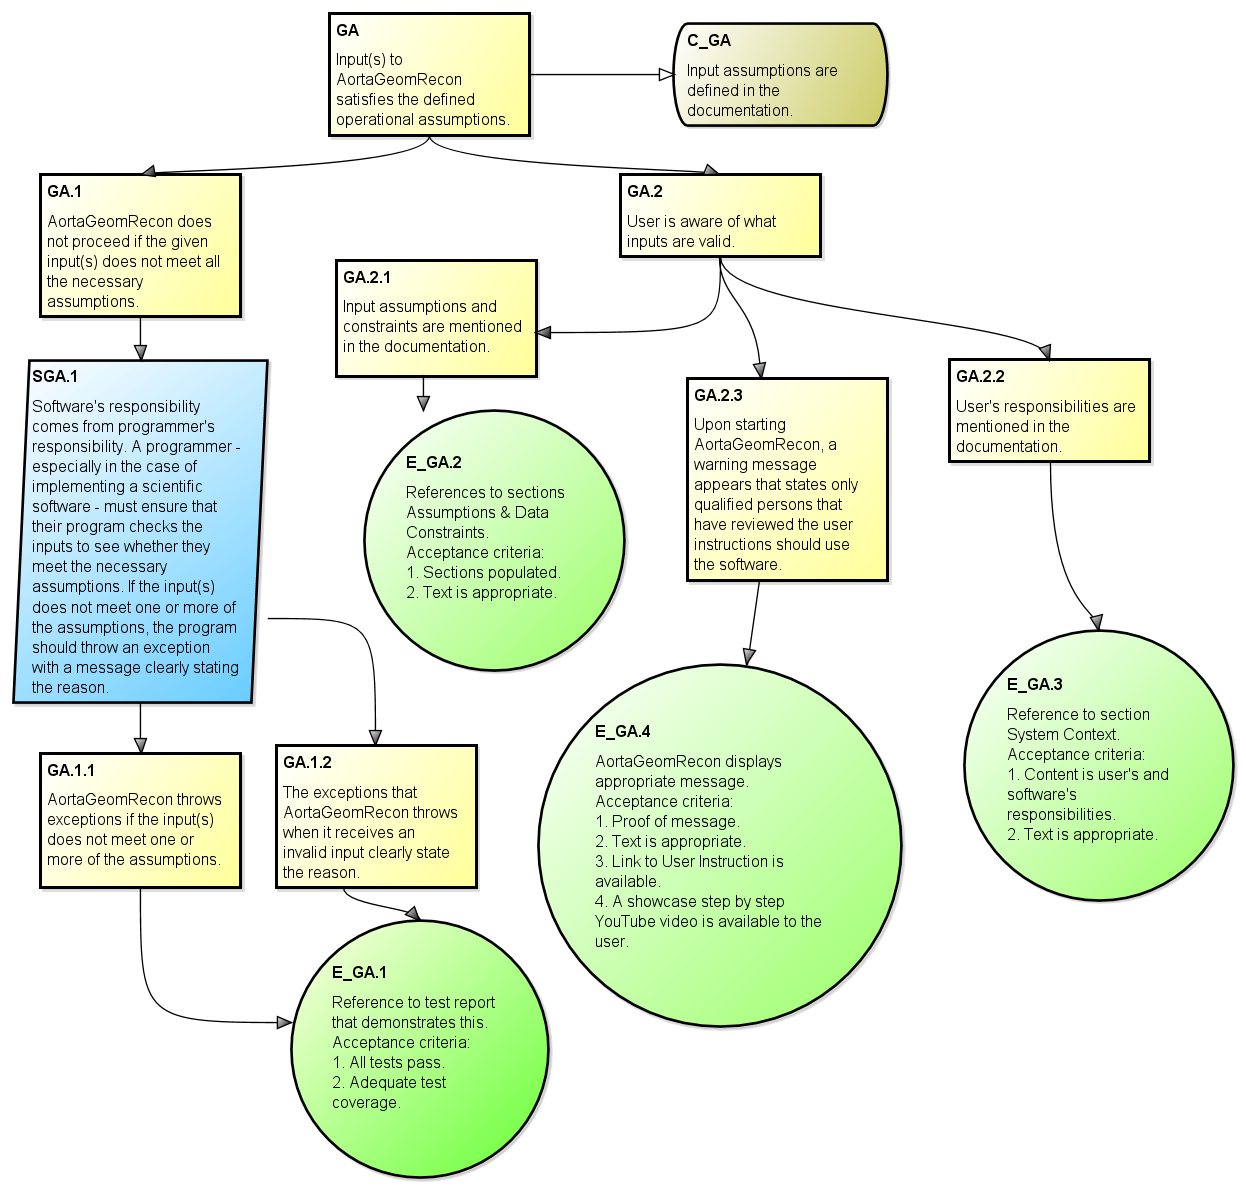
\includegraphics[width=\textwidth]{figures/AC/GA/GSN_GA.png}}
    \caption[AortaGeomRecon Assurance Case Inputs Assumptions]{AortaGeomRecon Assurance Case Inputs Assumptions}
    \label{fig_agr_ac_ga}
\end{figure}

This statement requires the user know what inputs are valid, and only used the valid inputs in the software.

\subsection{Warning Message}

As we initially planned, this piece of information is available in the User Manual and User Instruction Video, where we showed the user how to import DICOM patient's data, and operate on the inputs' data till we get a segmentation result. A user who has read the User Manual and watched the instruction video should know what inputs are valid. Therefore, in the AortaGeomRecon module, we need to effectively guide the user to the User Manual, whether the user has used this software before or it is a first time user.

\begin{figure}[H]
    \centering
    \fbox{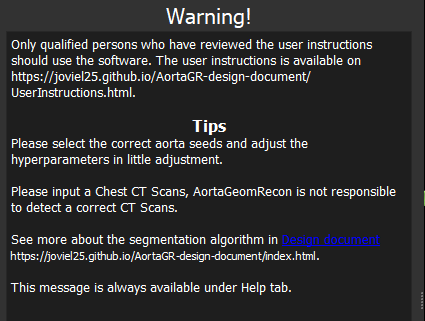
\includegraphics[width=0.6\textwidth]{figures/AC/GA/AGR_warning.png}}
    \caption[AortaGeomRecon Warning Message]{AortaGeomRecon Warning Message}
    \label{fig_agr_ac_wm}
\end{figure}

As mentioned in the section \ref{module_workflow}, when the user first starting 3D Slicer and click on the AGR module, this warning message appears. The user must clicks on the Confirm button to continue to the next steps. With the warning message shown to the user, it is now the user's responsibility to use the valid inputs for AGR, which the program will deliver the correct outputs if the other operations are performed correctly. 

%Here is a sample equation (Equation~\ref{eq_lineslope}):
%
%\begin{equation} \label{eq_lineslope}
%	y = mx + b
%\end{equation}